\section{実験結果および考察} \label{sec5}
\subsection{ランキングモデルの性能評価} \label{sec5.1}
~\ref{Evaluation_of_Ranking_Prediction_Results}にRMの性能評価の結果を示す．
目的変数ごとに，太字は一番高い値，下線は次に高い値を示す．
全ての目的変数において，LightGBM，XGBoost，CatBoostはベースライン手法を上回っており，上位候補の提示に有効であることが確認された．
% 特に，モデル間の比較では，適合率，再現率，$F_1$値，時間のいずれの目的においても，LightGBMがNDCG@KおよびHit@Kで最良となる事例が多かった．
モデル間の比較において，LightGBMは全12通りの実験のうち10通りで，NDCG@KおよびHit@Kで最良の結果を示した．
LightGBMにおけるNDCG@1は，適合率・再現率・$F_1$値の予測で 67.15～71.46\%，実行時間の予測で 99.71\% を示した．
また，HitはKの増加に伴い上昇しており，最良候補を上位K件に含めるという観点で安定した性能を示した．
以上より，評価項目(ii)と(iii)ではLightGBMを採用する．

\begin{table}[tb]
 \caption{ランキングモデルの性能評価の結果}
 \label{Evaluation_of_Ranking_Prediction_Results}
 \centering
 \footnotesize
% \resizebox{\columnwidth}{!}{
 \begin{tabular}{llrrrrrr}
    \toprule
    目的 & モデル & NDCG@1 & NDCG@5 & Hit@1 & Hit@5 \\
    \midrule
    \multirow{4}{*}{P}
     & LightGBM & \textbf{67.15}  & \textbf{68.48} & \textbf{60.00} & \textbf{70.00} \\
     & XGBoost  & \textbf{67.15}  & \underline{66.53} & \textbf{60.00} & \textbf{70.00} \\
     & CatBoost & \underline{64.18}  & 65.29 & \underline{56.25} & \underline{68.75} \\
     & ランダム & 22.29  & 23.05 & 16.13 & 39.88  \\
    \midrule
    \multirow{4}{*}{R}
     & LightGBM & \textbf{71.46}  & \textbf{72.07} & \textbf{48.75} & \underline{60.00} \\
     & XGBoost  & \underline{69.55} & \underline{70.94} & \textbf{48.75} & \textbf{61.25} \\
     & CatBoost & 65.96 & 67.45 & \underline{40.00} & 55.00 \\
     & ランダム & 33.47 & 34.37 & 8.63 & 32.00 \\
    \midrule
    \multirow{4}{*}{$F_1$}
     & LightGBM & \textbf{68.52} & \textbf{67.81} & \textbf{56.25} & \textbf{65.00} \\
     & XGBoost  & 61.95& 64.00 & \underline{48.75} & \underline{63.75} \\
     & CatBoost & \underline{64.39} & \underline{65.74} & 47.50 & 60.00 \\
     & ランダム & 22.67  & 23.32 & 10.75 & 36.13 \\
    \midrule
    \multirow{4}{*}{T}
     & LightGBM & \textbf{99.71}  & \textbf{99.54} & \underline{81.25}  & \textbf{100.00} \\
     & XGBoost  & 99.39  & \underline{99.53} & 72.50 & \textbf{100.00} \\
     & CatBoost & \underline{99.55} & \textbf{99.54} & \textbf{82.50} & \textbf{100.00} \\
     & ランダム & 50.56 & 51.75 & 1.88 & \underline{10.50} \\
    \bottomrule
    \end{tabular}
%    }
\end{table}

\subsection{選択されたRAG構成を用いたRAGの性能評価} \label{sec5.2}
\ref{Evaluation_of_RAG_Based_on_Selection_Results}に選択されたRAG構成を用いたRAGの性能評価の結果を示す．
%ランキング上位K件（$@1$，$@5$）からRAG構成を選択する場合の性能を，五つの重み設定および各ベースライン手法と比較した結果を示す．
標準設定においては，適合率が38.61\%，再現率が51.76\%，$F_1$値が40.50\%，時間が5.18秒であった．
提案@1の$F_1$値-時間は，標準設定と比較して，適合率を2.46\%，再現率を3.26\%，$F_1$値を3.08\%改善しつつ，時間を3.75秒短縮した．
また，提案@1の時間重視は時間が1.41秒であり，標準設定と比較して3.77秒短縮した．
最頻出設定においては，適合率が40.94\%，再現率が55.02\%，$F_1$値が43.55\%，時間が1.41秒であり，提案@1の時間重視の1.41秒と同値であった．
ランダム選択においては，適合率が0.06\%，再現率が23.37\%，$F_1$値が8.20\%，時間が51.29秒であり，提案@1と比較して精度が低下し，コストも増加した．

\begin{table}[tb]
 \caption{選択されたRAG構成を用いたRAGの性能評価の結果}
 \label{Evaluation_of_RAG_Based_on_Selection_Results}
 \centering
 \footnotesize
 \begin{tabular}{ccrrrr}
    \toprule
    \multicolumn{2}{c}{手法} & 適合率 & 再現率 & $F_1$値 & 時間(秒) \\
    \midrule
    \multirow{5}{*}{提案@1} 
    & $F_1$値-時間 & 41.07 & 55.02 & 43.58 & \underline{1.43} \\
    & 適合率重視 & 39.16 & 52.03 & 41.55 & 5.49 \\
    & 再現率重視 & \textbf{43.85} & \textbf{57.05} & \textbf{46.25} & 9.88 \\
    & $F_1$値重視 & 42.12 & \underline{56.44} & 45.08 & 7.24 \\
    & 時間重視 & 40.94 & 55.02 & 43.55 & \textbf{1.41} \\
    \midrule
    \multirow{5}{*}{提案@5} 
    & $F_1$値-時間 & 40.18 & 54.64 & 43.11 & 4.83 \\
    & 適合率重視 & 39.01 & 53.20 & 41.86 & 7.10 \\
    & 再現率重視 & \underline{42.37} & 56.36 & \underline{45.33} & 8.79 \\
    & $F_1$値重視 & 40.63 & 55.69 & 43.67 & 8.99 \\
    & 時間重視 & 30.57 & 46.10 & 33.57 & 2.16 \\
    \midrule
    \multicolumn{2}{c}{標準設定} & 38.61 & 51.76 & 40.50 & 5.18 \\
    \multicolumn{2}{c}{最頻出設定} & 40.94 & 55.02 & 43.55 & \textbf{1.41} \\
    \multicolumn{2}{c}{ランダム選択} & 0.06 & 23.37 & 8.20 & 51.29 \\
    \midrule
    \multirow{4}{*}{オラクル}
    & 適合率最良 & 55.08 & 68.17 & 58.05 & 14.91 \\
    & 再現率最良 & 51.36 & 72.46 & 58.04 & 14.91 \\
    & $F_1$値最良 & 53.83 & 70.38 & 59.72 & 15.90 \\
    & 時間最良 & 40.86 & 54.99 & 43.49 & 1.27 \\
    \bottomrule
    \end{tabular}
%    }
\end{table}

\subsection{ユーザを考慮したRAG構成選択の性能評価} \label{sec5.3}
\ref{Evaluation_of_RAG_Based_on_Selection_Results_max}にユーザを考慮したRAG構成選択の性能評価の結果を示す．
%提案手法においてランキング上位K件（@3，@5）からRAG構成を選択する場合の性能を，5種類の重み設定で比較した結果を示す．
まず提案@3では，再現率重視においては，適合率が44.70\%，再現率が59.37\%，$F_1$値が48.68\%，時間が9.88秒であり，適合率と$F_1$値で最も高かった．
また，$F_1$値重視においては，適合率が44.46\%，再現率が59.46\%，$F_1$値が47.68\%，時間が7.78秒であり，再現率が最も高かった．
一方，時間重視においては，適合率が41.17\%，再現率が55.18\%，$F_1$値が43.75\%，時間が1.27秒であり，時間が最も短かった．
次に，\ref{Evaluation_of_RAG_Based_on_Selection_Results}に示すオラクルと比較する． 
まず，提案@3と@5の時間重視において，時間がオラクルの時間最良設定と一致した．
提案@5の時間重視においては，適合率と再現率と$F_1$値も一致した．
一方，オラクルの適合率最良構成，再現率最良構成，$F_1$値最良構成と提案手法との間に差は存在する．
提案@5の$F_1$値重視において，適合率が45.40\%，再現率が62.19\%，$F_1$値が50.25\%であり，オラクルの$F_1$値最良構成とはそれぞれ，適合率が8.43\%，再現率が8.19\%，$F_1$値が9.47\%の差がある．

\begin{table}[tb]
 \caption{ユーザ選択を含むRAG構成の性能評価の結果}
 \label{Evaluation_of_RAG_Based_on_Selection_Results_max}
 \centering
 \footnotesize
 \begin{tabular}{ccrrrr}
    \toprule
    \multicolumn{2}{c}{手法} & 適合率 & 再現率 & $F_1$値 & 時間(秒)  \\
    \midrule
    \multirow{4}{*}{提案@3} 
    & 適合率重視 & \underline{44.47} & 56.67 & 46.86 & \underline{6.20} \\
    & 再現率重視 & \textbf{44.70} & \underline{59.37} & \textbf{48.68} & 9.88 \\
    & $F_1$値重視 & 44.46 & \textbf{59.58} & \underline{47.68} & 7.78 \\
    & 時間重視 & 41.17 & 55.18 & 43.75 & \textbf{1.27} \\
    \midrule
    \multirow{4}{*}{提案@5} 
    & 適合率重視 & 45.24 & 58.42 & 48.03 & \underline{6.82} \\
    & 再現率重視 & \textbf{46.41} & \underline{60.93} & \textbf{50.53} & 7.13 \\
    & $F_1$値重視 & \underline{45.40} & \textbf{62.19} & \underline{50.25} & 7.76 \\
    & 時間重視 & 40.86 & 54.99 & 43.49 & \textbf{1.27} \\
    \bottomrule
    \end{tabular}
\end{table}


\subsection{考察} \label{sec5.4}
提案手法の有効性は以下の3点に集約される．
1点目は，RM学習により有望な設定を上位に集約できる点である．
2点目は，重み付き統合によって運用目標に応じたトレードオフ制御が可能である点である．
本手法は式~\eqref{eq1}のように，各指標の順位の逆数を用いて定式化している．
この定式化では，特定の指標が支配的となり，他の指標の影響が無視される懸念があった．
しかし，\ref{Evaluation_of_RAG_Based_on_Selection_Results}の通り，設定した重みに応じてトレードオフは機能しており，特定の指標のみに依存しないことを確認した．
したがって，順位の逆数を用いた単純加算による定式化は，RAG構成の選択において効果的である．
3点目は，単一のRAG構成だけでなく，複数の構成を上位候補集合としてユーザに提示することで，実運用における頑健性を高められる点である．
コストを重視した設定に関してはオラクル近傍の性能が得られており，実用上の価値がある．
これらの結果は，単一の構成を予測するのではなく，優れた候補集合を提示してユーザが事後的に選択する設計が，適応的なRAGの実運用において現実的であることを示唆している．
この設計により，候補数Kを増やしても性能が単調に改善しないという欠点を，ユーザの手動調整によって補完できる．
% これらの結果は，適応的なRAGの実運用において，単一の構成を予測するのではなく，優れた候補集合を提示し，ユーザが回答を事後的に選択することによって性能を最大化する設計が現実的であることを示している．

\subsection{アブレーション分析} \label{sec5.5}
%一部の特徴量のみを用いた学習結果を分析した．
アブレーション分析として，RAG構成，質問の表層的特徴，文書の表層的特徴量，および意味的特徴量を用意し，それらを単独または複数組合せて入力した場合の性能を比較する．
学習にはLightGBMを用い，$F_1$値を目的変数とした場合のランキング予測性能を評価する．
評価にはNDCG@1，NDCG@5，Hit@1，およびHit@5 を用いる．

\ref{tab:feature_ablation_ndcg_hit}にアブレーション分析結果を示す．
太字は一番高い値，下線は次に高い値を示す．
1観点の特徴量のみを用いた場合ではRAG構成（C）が最も高く，NDCG@1が66.84\%，Hit@5が62.50\% を示した一方で，質問の表層的特徴量（Q），文書の表層的特徴量（D）および意味的特徴量（S）はNDCG@1 が 21.90\%～26.42\%，Hit@5 も21.25\%～23.75\% に留まった．
この結果は，RAG構成がランキング予測における主要因であることを示している．
RAG構成を含まない組合せは，総じて低性能である．
特に，3観点の特徴量を組み合わせた場合でも NDCG@1が23.27\%，Hit@5が32.50\% に留まった．
このことから，質問や文書の内容情報だけでは高精度な順位付けが難しいことが示唆される．
一方で，RAG構成に他の特徴量を追加すると性能が改善する傾向が見られた．
RAG構成と質問の表層的特徴量と意味的特徴量は NDCG@1が64.94\%，Hit@5が61.25\%，RAG構成と質問の表層的特徴量と文書の表層的特徴量はNDCG@1が62.15\%，Hit@5が60.00\% と比較的高い値を示した．
最終的に，提案手法が最良となり，NDCG@1が68.52\%，Hit@5が65.00\% を達成した．

以上の結果から，RAG構成が性能を規定する一方で，表層的特徴量と意味的特徴量を統合することで上位候補の選択がさらに改善され，提案手法が最も高いランキング性能を実現することが確認された．

% \begin{table}[tb]
%  \caption{アブレーション分析結果}
% RC & QSu & DSu & Se
\begin{table}[tb]
 \caption{RAG構成（C）・質問の表層的特徴量（Q）・文書の表層的特徴量（D）・意味的特徴量（S）のアブレーション分析結果}
 \label{tab:feature_ablation_ndcg_hit}
 \centering
 \footnotesize
% \resizebox{\columnwidth}{!}{
 \begin{tabular}{ccccrrrr}
  \toprule
  C & Q & D & S & NDCG@1 & NDCG@5 & Hit@1 & Hit@5 \\
  \midrule
  \ding{51} & - & - & - & \underline{66.84}  & \textbf{68.33} & \textbf{56.25} & \underline{62.50} \\
  - & \ding{51} & - & - & 23.29 & 23.62 & 18.75 & 26.25 \\
  - & - & \ding{51} & - & 26.42 & 26.82 & 15.00 & 27.50 \\
  - & - & - & \ding{51} & 21.90 & 22.81 & 16.25 & 23.75 \\
  \midrule
  \ding{51} & \ding{51} & - & - & 63.81 & 63.88 & 51.25 & 58.75 \\
  \ding{51} & - & \ding{51} & - & 60.66 & 62.44 & 47.50 & 58.75 \\
  \ding{51} & - & - & \ding{51} & 60.82 & 62.58 & 47.50  & 61.25 \\
  - & \ding{51} & \ding{51} & - & 25.62 & 26.27 & 15.00 & 27.50 \\
  - & \ding{51} & - & \ding{51} & 23.16 & 22.98 & 18.75 & 25.00 \\
  - & - & \ding{51} & \ding{51} & 23.56 & 24.46 & 12.50 & 26.25 \\
  \midrule
  \ding{51} & \ding{51} & \ding{51} & - & 62.15 & 64.69 & 50.00 & 60.00 \\
  \ding{51} & \ding{51} & - & \ding{51} & 64.94 & 65.53 & \underline{52.50} & 61.25 \\
  \ding{51} & - & \ding{51} & \ding{51} & 62.07 & 62.99 & 47.50 & \underline{62.50} \\
  - & \ding{51} & \ding{51} & \ding{51} & 23.27 & 24.44 & 16.25 & 32.50 \\
  \midrule
  \ding{51} & \ding{51} & \ding{51} & \ding{51} & \textbf{68.52} & \underline{67.81} & \textbf{56.25} & \textbf{65.00} \\
  \bottomrule
 \end{tabular}
% }
\end{table}


\subsection{特徴量分析} \label{sec5.6}
LightGBMを用いて学習したRMにおける特徴量の貢献度を分析した．
これにより，ランキング決定に強く関与する特徴量群を特定し，RAG構成と質問・文書由来の特徴量との相対的な影響度を定量的に比較した．

% 特に，RAG構成以外の特徴量が同等以上の貢献度を持つ場合，提案手法が「RAG構成」だけでなく，「質問や文書の難易度や情報要求」といった入力依存の信号を利用して選択していることが示唆される．
% 図~\ref{feature_importance_f1_LightGBM_final}に，LightGBMを用いた特徴量の貢献度分析の結果を示す．
生成モデルの貢献度が約23\%と最大であり，検索方法（約20\%）とRAG（約8\%）がそれに次ぐ結果となった．
生成モデルと検索方法というRAG構成に関する特徴は，$F_1$値を最大化するランキング決定において支配的である．
RAG構成以外の特徴も寄与を示しており，文書のトークン数（約13\%）や質問と文書のコサイン類似度（約9\%）が上位に位置する．
文書の長さや質問と文書の類似度から得られる応答の難易度は，設定の選択に影響を及ぼしている．
質問タイプ（約7\%）や質問・文書間の固有表現に基づくコサイン類似度（約7\%）も上位に含まれる．
RMは，質問と文書から得られる情報や対応関係を手がかりとして順位付けしている．
一方で，チャンクサイズ（約2\%）やチャンクオーバーラップ（約1\%）といったRAG構成の寄与は小さい．

本分析を通じて特徴量選定の根拠を明確化し，RAG構成のみに基づく選択では不十分であること，および質問・文書由来の特徴量の組み込みがランキング予測に寄与することを示した．

% \begin{figure*}[htbp]
% \centerline{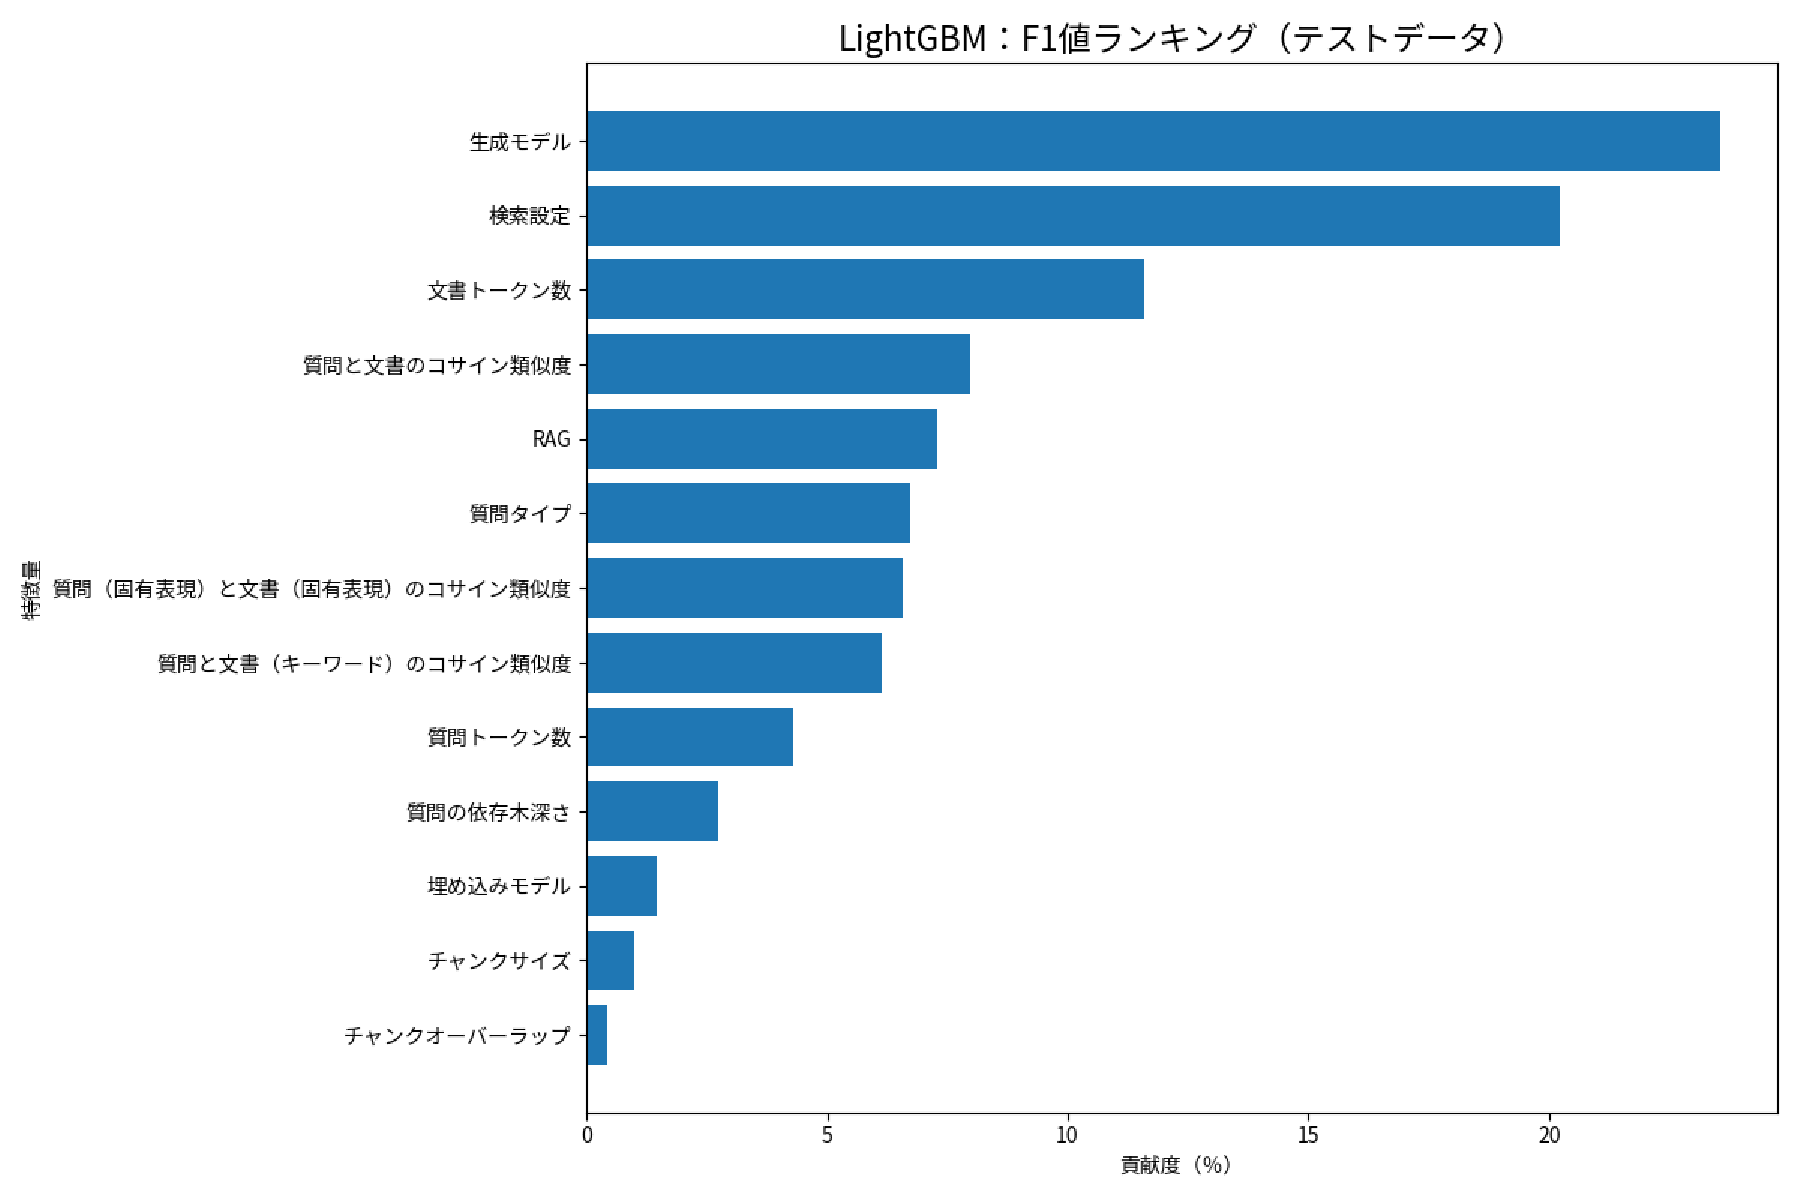
\includegraphics[width=\linewidth]{figures/feature_importance_f1_LightGBM_final.pdf}}
% \caption{$F_1$値ランキングにおける特徴量の貢献度}
% \label{feature_importance_f1_LightGBM_final}
% \end{figure*}

\subsection{定性分析} \label{sec5.7}
二つの質問応答例を用い，提案手法の挙動と失敗要因を定性的に分析する．
まず，映画監督の卒業大学を問う質問「Where did the director of film Nalini By Day, Nancy By Night graduate from?」を例に挙げる．
最頻出設定では「temple university」が得られ，提案@1でも同様に「temple university」を出力した．
続く提案@2から@4の設定も同様にNaiveRAGベースの構成であり，同様の誤答が出力された．
一方で，提案@5には異なる設定が含まれ，その実行結果として「mount holyoke college」のような正解となる回答が生成された．
これは，上位候補を広げるほど探索空間が拡大するためで，提案手法は固定のRAG構成では得ることのできない別回答を，候補集合として提示可能であることを示した．

次に，映画監督の死亡時期を比較する質問「Which film has the director died later, The Life And Loves Of Tschaikovsky or Dokuz Dağın Efesi?」を例に挙げる．
オラクルではGraphRAG構成で最大となる$F_1$値を示したが，$F_1$値RMはNaiveRAG構成を上位と予測した．
本質問は時系列的な事実照合を要し，複数文書間の関係をたどる必要がある．
GraphRAGは文書間関係を表現できるため，本来はこの種の質問に適する．
一方で，NaiveRAGは局所的な文脈一致に強く，質問と文中の単語レベルの類似度が高い場合に過大評価される傾向がある．
RMがコサイン類似度やトークン数といった特徴に影響され，GraphRAGよりもNaiveRAGを誤って選択したと推察される．

\subsection{本研究の限界} \label{sec5.8}
本研究では，RM学習により低コストかつ適応的なRAG構成選択を実現したが，以下の限界がある．

第一に，本手法は質問と文書の表層的および意味的特徴量である計7種を採用した．
定性分析の結果，高度な時系列推論や複数文書にまたがる複雑な論理構造を要する質問に対し，RMがNaiveRAGを誤選択する事例を確認した．
これは，現在の特徴量が語彙的類似性や文構造の深さに依存しており，知識グラフの構造的な適合性を評価できていないことに起因する．

第二に，本手法は実行時間の短縮において，オラクルに近い性能を達成した．
一方で，適合率や$F_1$値の最大化については，依然としてオラクル構成との間に有意な差がある．
96通りの構成空間において，精度を最大化する構成が局所的であり，現在のRM学習ではこれらを捉えきれていない可能性が高い．

第三に，大規模な実測データを効率的に収集するため，自動評価指標であるBERTScoreを用いた．
BERTScoreは意味的な類似性の評価に優れるが，コンテキストの忠実性やハルシネーションの有無を直接的には評価しない．
そのため，RMが事実とは異なる回答を生成する構成を高く評価するリスクを排除できていない．

第四に，本実験はSQuADおよびHotpotQAなどの一般的なドメインを用いて検証したが，医療，法務，社内文書といった専門性の高いドメインにおける有効性は未検証である．
文書の専門性や用語の特異性が高い場合，現在の埋め込みモデルに基づく意味的特徴量が機能しない可能性がある．
また，本手法はオフライン学習を対象としているため，未知のドメインデータを追加した際の有効性は保証されない．